\chapter{Modellentwurf}\label{sec:modellentwurf}
Nachdem nun alle notwendigen Grundlagen erläutert wurden, wird in diesem Kapitel der Grid Fin samt Aktuatorik entworfen. Hierzu werden zunächst die Anforderungen an das System aufgestellt, um dann auf dieser Basis eine geeignete Wahl der Designvarianten treffen zu können. Zur Übersicht über die verschiedenen technischen Umsetzungsvarianten wird ein morphologischer Kasten zur Hilfe gezogen. Schlussendlich wird in Abschnitt \ref{sec:modelldesign} ein erstes Modell zusammengestellt und anschließend in CAD modelliert.
\section{Systemanforderungen}
Zunächst werden also die Anforderungen an das System definiert. Hierbei wird sich hauptsächlich auf eine in MatLab mit Simulink durchgeführte Simulation und Angaben von GAIA Aerospace bezogen.
\subsection{Leistungsanforderungen}
Das wichtigste ist natürlich, dass die Grid Fins ihre Funktion erfüllt, beim Wiedereintritt einen stabilen Flug zu gewährleisten. Simulationen haben ergeben, dass hierfür ein Beiwertanstieg von $C_{N\alpha} =0,048/^\circ=2,75/$rad und einer Fläche $A=0,09\mathrm{m}^2$. Die zu entwerfenden Finnen sollten also vergleichbare Normalkräfte produzieren können.

Auch wenn die Axialkraft zusätzlich zur Stabilität beiträgt, ist sie weniger wichtig und liegt in den bisherigen Simulationen bei $C_X=0,1$ bei $\mathrm{Ma}_\infty=$ und $\alpha=0$. Generell ist sie jedoch positiv zu bewerten, da je größer der Aerodynamische Widerstand der Grid Fins ist, desto sicherer ist unversehrte der Flug und die Triebwerke, die den größten Anteil zur aerodynamischen Bremsung leisten, werden geschont. Dies sollt jedoch nicht auf Kosten der Lebensdauer der Grid Fins passieren, weil sonst der Aspekt der Wiederverwendbarkeit eingeschränkt wird.
\\~\\
Die Aktuatoren müssen nun gewährleisten, dass die Grid Fins zu jedem Zeitpunkt unter gegebener Last die notwendige Position einnehmen können. Für den Klappwinkel sind die Anforderungen an den Motor und das zugehörige Getriebe also sehr gering. Die Bewegung passiert hier ohne angreifende Kräfte, sodass nur die eigene Trägheit und die Lagerreibung überwunden werden muss. Dabei ist auch keine hohe Drehrate erforderlich, da für dieses Manöver theoretisch der gesamte Zeitraum zwischen Separation und Wiedereintritt zur Verfügung steht. Die restliche Zeit muss nur dafür gesorgt werden, dass die Grid Fins diese Position halten. Der aerodynamische Widerstand wirkt hierbei sogar unterstützend mit, die aus den Trägheitskräften resultierenden Moment um dieses Gelenk müssen jedoch standgehalten werden.
Der Klappwinkel muss also einmal von $\Lambda=90^\circ$ zu $\Lambda=0^\circ$ bewegbar sein und sich dort halten lassen

Der Aktuator für das Steuergelenk muss dagegen deutlich höhere Leistungen aufbringen. Der Steuerwinkel wird während des Wiedereintritts ständig vom Regler verändert. Somit kommen zu den Trägheits- und Reibungskräften auch noch die aerodynamischen Kräfte hinzu. Wenn auch deutlich größer sind sie zu planaren Finnen jedoch vergleichsweise gering, wie in dem vorherigen Kapitel gezeigt wurde. Im Gegensatz zum Klappwinkel spielt hier auch die Drehrate eine wichtige Rolle, da nur, wenn die Grid Fins auch schnell genug reagieren, kann der Flug effizient geregelt werden. In der Simulink-Simulation kommt es bei unbeweglichen Grid Fins zu Schwingungen in der aerodynamischen Flugphase mit einer Periodendauern von $\Delta t=0,73$s. Um diese auszugleichen, muss also auch der Steuerwinkel in der selben Zeit vom maximalen Ausschlag in die eine Richtung zum maximalen Ausschlag in die andere und wieder zurück drehen können. Da der Steuerwinkel im Bereich $\eta = [-20^\circ,20^\circ]$ liegen soll, folgt nun also eine durchschnittliche Drehrate von mindestens $109,59^\circ/\mathrm{s}=1,913\mathrm{rad/s}$ erreicht werden.
\subsection{Anforderungen an die Kosten}
Für die Kosten gilt das klare Ziel diese zu Minimieren und somit maximale Wirtschaftlichkeit zu erreichen. Somit sollen so weit es geht COTS verwendet werden, die keine teure Sonderanfertigung benötigen. Kleine Bauteile sparen sogar doppelt Geld, da sie zum einen weniger Materialkosten haben und zum anderen für den Flug der Rakete ihr Gewicht weniger erhöhen, sodass geringere Mengen an Treibstoff benötigt beziehungsweise mehr Nutzlast mitgenommen werden kann.
\subsection{Thermische und Mechanische Anforderungen}
Beim Wiedereintritt treten sehr hohe thermische Lasten auf, die sich jedoch schwer im Vorfeld quantifizieren lassen, da sie stark von der Geometrie abhängen und sich nur durch aufwendige CFD-Simulationen bestimmen lassen. Generell gilt für die thermische Belastung, dass umströmte Fläche, besonders an der Vorderkante, einen negativen Effekt hat und die Wärme des durch den Verdichtungsstoß stark erhitzen Fluids aufnimmt. Währenddessen ist ein großes Volumen mit idealer Weise hoher Wärmekapazität vorteilhaft, da dieses die Energie der Außenfläche aufnehmen kann. Dieser Effekt ist am besten bei hoher Wärmeleitfähigkeit nutzbar und sorgt für möglichst geringe Temperaturgradienten, die wiederum auch Eigenspannungen verursachen würden. Am wichtigsten ist jedoch die Schmelztemperatur, beziehungsweise die maximale Temperatur, bei der der Werkstoff noch akzeptable mechanische Eigenschaften hat, weil dies schlussendlich bestimmt wie viel Wärme ausgehalten werden kann.
\\~\\
Für die Stabilität gilt, dass sich die Grid Fins und natürlich auch ihre Aktuatorik nicht plastisches Verformen oder gar vollständig versagen darf. Dabei ist auch besonders auf das Kriechen zu achten, welches bei einer Kombination von thermischer und mechanischer Belastung wie sie hier vorliegt schnell auftreten kann.

Abbildung \ref{abb_KraefteNormal} zeigt die an einem der vier Grid Fins angreifenden Kräfte im Körperfesten System bei einer Mission der Valkyrie, wenn sie durchgehend in der Neutralstellung gehalten und nicht gesteuert oder geregelt werden. Dargestellt sind sowohl die Kräfte in negative X-Richtung (rot), als auch in Y- (blau) und Z-Richtung (grün) im Zeitintervall von $t=400$s bis $t=500$s nach der Entkoppelung von den Pylonen. Während die Axialkraft relativ monoton steigt und fällt sind die Normalkräfte starken Schwankungen auf Grund der Abwesenheit eines Reglers ausgesetzt.

Es ist zu erkennen, dass bei ungefähr $t=400$s der Wiedereintritt beginnt und die Kräfte anfangen zu steigen. Diese schwellen schnell auf und der Lastenvektor $\vec{F}$ erreicht seinen Höhepunkt bei
\begin{equation}
	\vec{F}(t=448,5\mathrm{s})=
		\left(\begin{array}{c}F_{-x}\\F_y\\F_z\end{array}\right)
			=\left(\begin{array}{c}487\mathrm{N}\\70\mathrm{N}\\220\mathrm{N}\end{array}\right).
\end{equation}
An dieser Stelle ist der Maximale Staudruck "Max Q"\ erreicht und wird für die Auslegung von entscheidender Bedeutung sein. Danach nehmen alle Kräfte wieder ab, da sich die Geschwindigkeit verlangsamt. 
\begin{figure}[h]
	\centering
	\includegraphics[width=0.9\textwidth]{FNormal.png}
	\caption{Kräfte an einem der Grid Fins bei konstant gehaltener Neutralstellung}
	\label{abb_KraefteNormal}
\end{figure}\\
Dies kommt dadurch zustande, dass die Dichte der Umgebungsluft zwar monoton steigt, die Geschwindigkeit aber abnimmt. Diese ist in Abbildung \ref{abb_vNormal} für den selben Zeitbereich dargestellt. Am Anfang macht sich die Atmosphäre noch nicht stark bemerkbar, dort steigt sogar die Geschwindigkeit durch die Flugbahn leicht an. Es folgt der ReEntry-Burn, der die Rakete von $U_\infty \approx 25000$m/s auf etwas über $15000$m/s abbremst. Danach lässt sich der Widerstand in der Atmosphäre an dem weiteren Abfallen der Fluggeschwindigkeit erkennen, deren Zeit mit den Kräften in Abbildung \ref{abb_KraefteNormal} übereinstimmt. Diese Reduzierung der Geschwingkeit erklärt die Abnahme der aerodynamischen Kräfte an den Grid Fins. Bei ungefähr $t=456$s ist ein Knick in der Geschwindigkeitskurve zu erkennen, der den Zeitpunkt markiert, an dem ein Machzahl von 2 unterschritten wurde, sodass der Ballute auslöst. Dies mindert die Geschwindigkeit weiter drastisch ab, damit sich der Gleitschirm sicher öffnen kann. Der Zeitraum nach dem Ballonschirm ist für die Auslegung der Grid Fins uninteressant.
\begin{figure}[h]
	\centering
	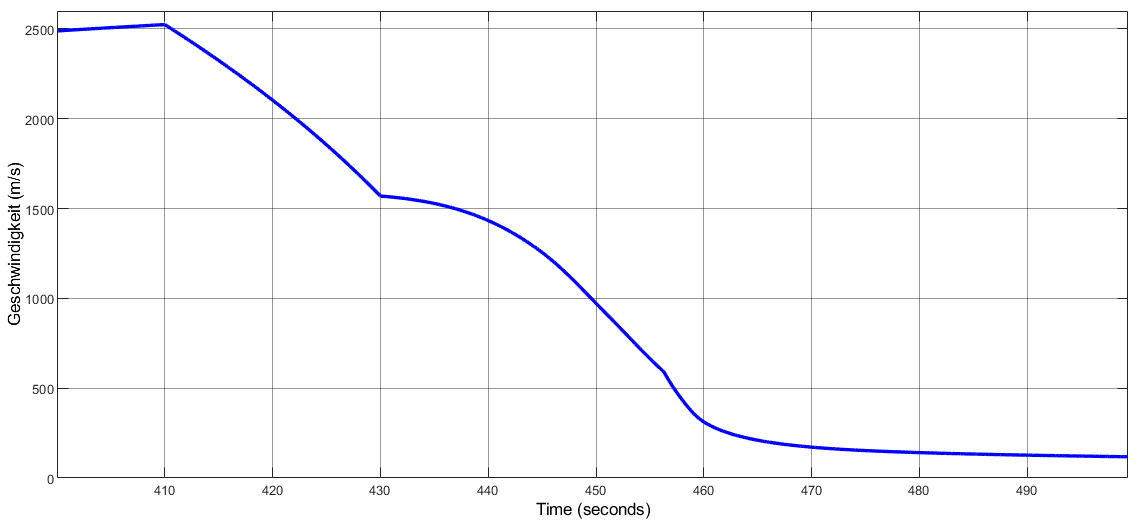
\includegraphics[width=0.9\textwidth]{vNormal.png}
	\caption{Fluggeschwindigkeit bei konstant gehaltener Neutralstellung}
	\label{abb_vNormal}
\end{figure}\\~\\
Dies war nun aber nur ein sehr simpler Missionsablauf, der den Grid Fins nicht viel abverlangt. Für die Auslegung müssen jedoch auch die worst-case-Szenarien berücksichtigt werden. Dazu zählt zum einem ein Ausschlag des Steuerwinkels, wodurch zum einem deutlich höhere Normalkräfte zu Stande kommen, aber auch die Axialkräfte deutlich ansteigen. Des Weiteren ist der Fall zu betrachten, dass der ReEntry-Burn ausfällt, beziehungsweise bewusst weggelassen wird, um die Wirtschaftlichkeit durch geringere Treibstoffmitnahme zu maximieren. In dem Fall würde die Raketenstufe mit deutlich höherer Geschwindigkeit in die Atmosphäre eintauchen, was zu enormen Belastungen führt.

Zu dem maximalen Lastfall kommt es, wenn kein ReEntry-Burn stattfindet und alle Grid Fins um $\eta = \pm 10^\circ$ ausgeschlagen sind. Die Finnen befinden sich dabei in x-Formation und der Ausschlag ist so ausgerichtet, dass ein Moment erzeugt wird, das den Nickwinkel erhöht. Die Kräfte, die in diesem Fall von den Grid Fins ausgehalten werden müssen sind für alle betragsmäßig gleich und in Abbildung \ref{abb_FExtreme} dargestellt. Während die Axialkraft nur leicht ansteigt, nehmen die Normalkräfte sehr hohe Werte an wie der Kraftvektor
\begin{equation}
	\vec{F}(t=440,7\mathrm{s})
	=\left(\begin{array}{c}817\mathrm{N}\\-6530\mathrm{N}\\-6183\mathrm{N}\end{array}\right)
\end{equation}
zeigt. Zu erkennen ist, dass der Wiedereintritt hochfrequenten Schwingungen ausgesetzt die Amplituden von bis zu $\Delta F_z = 3194$N besitzen. Wird nun aber davon ausgegangen, dass eine funktionstüchtige Reglung existiert, so kann diese Schwingung ausgeglichen werden und es käme ein Kraftvektor mit den Mittelwerten zu Stande.
\begin{equation}\label{eq_Fmax}
\vec{F}_\mathrm{geregelt}(t=440,7\mathrm{s})
=\left(\begin{array}{c}572\mathrm{N}\\-6415\mathrm{N}\\-4995\mathrm{N}\end{array}\right)
\end{equation}
Der Moment, in dem eine Machzahl von $Ma_\infty = 2$ erreicht qird und der Ballonschirm deployed, ist zwar in diesem Fall deutlich erkennbar, da die Raketenstufe in diesem Moment plötzlich herumgerissen wird, kann jedoch im Vergleich zu den Kräften bei "Max Q"\ vernachlässigt werden.
\begin{figure}[h] 
	\centering
	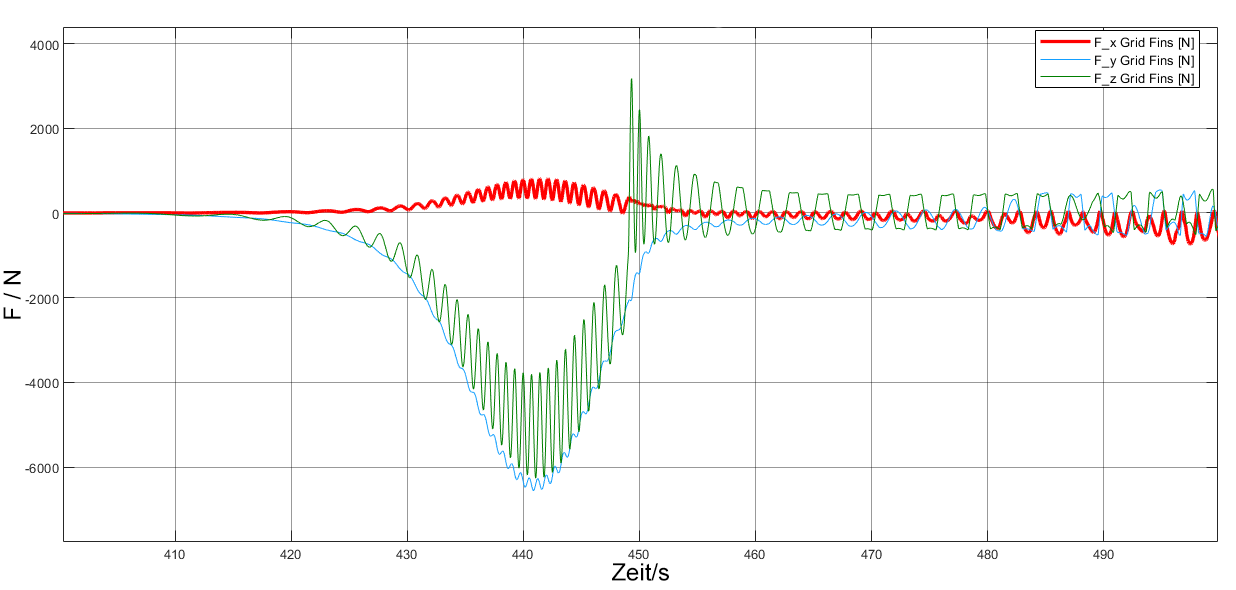
\includegraphics[width=0.9\textwidth]{F2Extreme4.png}
	\caption{Kräfte am Grid Fin beim maximalen Lastfall}
	\label{abb_FExtreme}
\end{figure}\\
\subsection{Geometrische Anforderungen}
Die Hauptmaße der Grid Fins sind hauptsächlich durch die Fertigung begrenzt. Ein Grid Fin soll also in einen entsprechenden 3D-Drucker mit den Maßen $300$x$300$x$400\mathrm{mm}^3$ passen. Für die Größe und Anordnung der Aktuatorik ist darauf zu achten, dass für alle vier Grid Fins jeweils zwei Motoren mit ihren zugehörigen Getrieben in den Raketendurchmesser von $1,1$m passen müssen. Das Innere dieses Durchmessers wird jedoch für die Bordelektronik benötigt, sodass sich die Aktuatorik am äußeren Rand befinden muss. Es ist des Weiteren eine Maximalhöhe von $0,15$m vorgesehen, die nicht überschritten werden darf.
\newpage
\section{Morphologischer Kasten}
Um eine Übersicht über die verschiedenen Designmöglichkeiten zu haben wird an dieser Stelle ein morphologischer Kasten, wie in er in Abbildung \ref{abb_MorphKastGF} zu sehen ist, eingeführt. Für fünf Designentscheidungen des Grid Fins sind dort unterschiedliche Teillösungen aufgelistet. Ganz links sind drei mögliche Zellformen gegeben. Es besteht die Wahl zwischen quadratischen, drei- und sechseckigen Geometrien. Hierbei sei aber wieder zu berücksichtigen, dass es auch zu einer Mischung mehrerer Formen kommen kann und besonders am Rand durch den Rahmen die Zellen ungleichmäßig verkleinert werden könnten.

Für die Form des gesamten Gitters stehen nur drei unterschiedliche Möglichkeiten zur Auswahl: Rechteck, Diamant oder auch eine dem Insektenflügel nachempfundene Struktur. Da jedoch die Maße noch nicht festgelegt sind kann die ersten der beiden Formen auch noch zum Quadrat werden. Des Weiteren kann es sein, dass die Geometrie an der einen Seite für die Anbringung noch angepasst wird.

Die größte Auswahl bietet sich bei den Wandquerschnittsformen. Rechteckig, abgerundet, beidseitig und einseitig spitzt, trapezförmig und dreieckig sind die sechs Optionen, die es hier gibt. Der Wandquerschnitt muss nicht überall die gleiche Form besitzen. So kann es kommen, dass das Gitter eine unterschiedliche erhält als der Rahmen. Die unteren beiden Formen sind zum Beispiel asymmetrisch, sodass sie nur für die Umrandung der Grid Fins in Frage kommen.

Als viertes wird die Fragestellung einer Krümmung gezeigt. Neben einem flachen Design kann der Grid Fin entweder zur Strömung hin konvex oder konkav gekrümmt sein. Dies ist abhängig davon in welche Richtung die Finne eingeklappt werden kann.

Im Grundlagenkapitel wurden drei verschiedene Arten der Pfeilung eines Grid Fins gezeigt. Da sie sich grundsätzlich unterschiedlich implementieren lassen, können sie theoretisch sogar in Kombination gewählt werden. Der Pfeilungswinkel ist für die Varianten noch frei wählbar und auch negative Winkel, also Vorwärtspfeilung, ist denkbar. Für die lokale Pfeilung der Zellen rückt der Unterschied zwischen Vorwärts- und Rückwärtspfeilung durch die Unterscheidung vom Berg- und Tal-Typus noch mehr in den Vordergrund. Wichtig ist noch anzumerken, dass die konfigurelle Pfeilung keinen direkten Einfluss auf das Design der Grid Fins an sich hat, sondern sich durch den Bewegungsspielraum der Aktuatorik umsetzten lässt.\\
Es gibt jedoch noch weitere Designentscheidungen, die sich nicht in einem morphologischen Kasten pragmatisch darstellen lassen. So müssen zum einen noch die Dimensionen des Moduls und Lage der Aktuatoren in der Rakete definiert werden. Zum anderen stellt sich die Frage welche Zellgröße $g$ und Wandstärke $d$ an welcher Stelle gewählt wird. Es besteht auch noch die Möglichkeit die Grid Fins mit zusätzlichen Features auszustatten. Eine Option wären hier zusätzliche Stützstreben oder sogar durch die additive Fertigung ermöglichte, in das Material integrierte Strukturen, wie zum Beispiel Kühlkanäle oder Drucksensoren.
\begin{figure}[h]
	\centering
	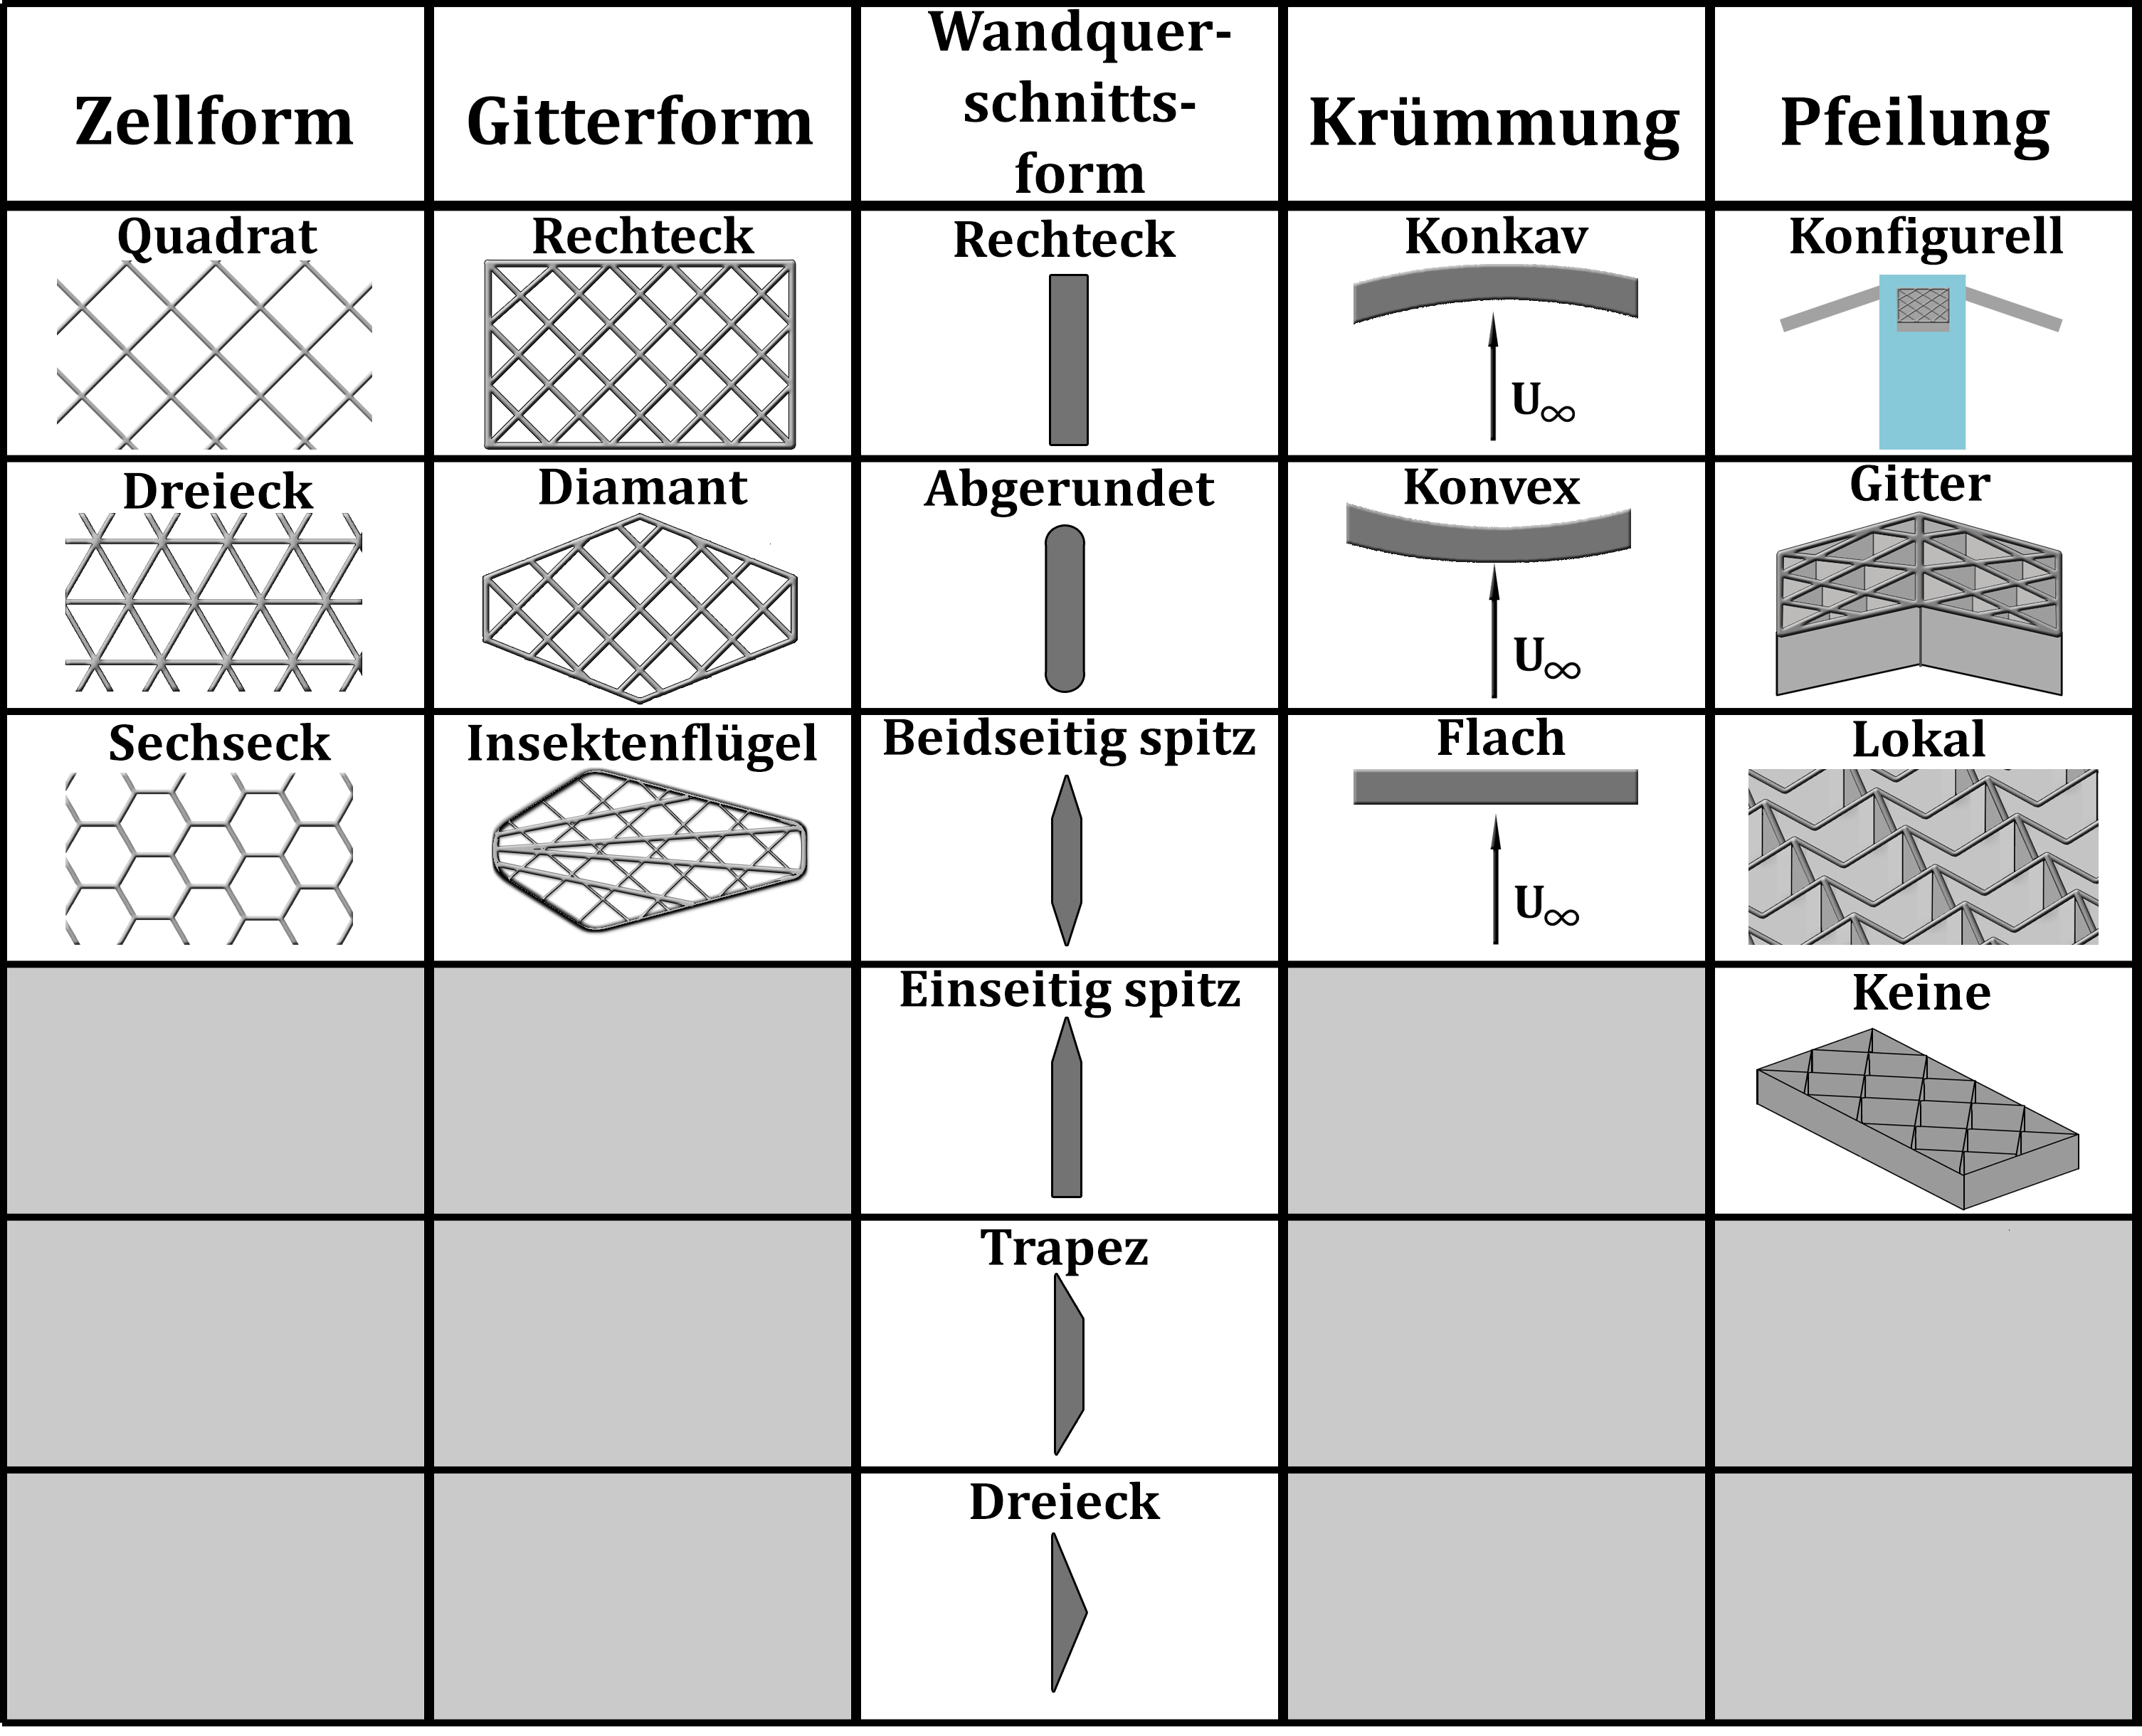
\includegraphics[width=0.9\textwidth]{Morphologischer Kasten GF V2.png}
	\caption{Morphologischer Kasten für die Grid Fins}
	\label{abb_MorphKastGF}
\end{figure}\\~\\
Für den Entwurf der Aktuatorik wurde ein zweiter morphologischer Kasten erstellt. Dieser ist in Abbildung \ref{abb_MorphKastAk} zu sehen und zeigt drei verschieden Designkategorien. Da die Grid Fins zwei unabhängige Freiheitsgrade haben, können für den Steuer- und Klappwinkel separat unterschiedliche Lösungen aus dem morphologischen Kasten gewählt werden.

Eine wichtige Designentscheidung ist der Aktuator, da er bestimmt was als Energiequelle genutzt wird und hat somit einen großen Einfluss auf Gewicht und Kosten. Eine Möglichkeit ist die elektrische Energie zu nutzen und diese mit einem Elektromotor direkt die mechanische Arbeit verrichten zu lassen. Hierbei muss noch die Wahl getroffen werden, ob linear oder rotatorischer Motor vorgezogen werden soll. Alternativ kann auch ein hydraulisches oder gar pneumatisches System verwendet werden. Da Grid Fins zwei Freiheitsgrade haben, können diese über unterschiedliche Aktuatoren, die auch unterschiedlicher Art sein können, bewegt werden. Also muss in diesem Punkt für beide Rotationen einzeln entschieden werden.

Über ein Getriebe wird die Leistung des Aktuators auf die Grid Fins übertragen, um mehr Spielraum für Kraft, Moment, Drehzahl und Orientierung des Aktuators zu gewährleisten. Eine Möglichkeit bietet das klassische Zahnradgetriebe. Viele Paarungen wie Stirn-, Kegel-, Schrauben- oder Schneckenräder sind denkbar. Kräfte und die zugehörige Bewegungsgeschwindigkeit lassen sich auch durch hydrostatische Getriebe beeinflussen. Momente und Drehzahlen können durch hydrodynamische Getriebe verändert werden. Generell sind durch Kombinationen beliebig komplexe Systeme möglich.

Als letztes beschäftigt sich der Morphologische Kasten in Abbildung \ref{abb_MorphKastAk} mit der Lagerung. Hierbei wird generell zwischen den Wälz- und Gleitlagern unterschieden. Beide bieten jedoch noch mehr Entscheidungsfreiheiten. So gibt es einige unterschiedliche Wälzkörper, wie Kugeln, Zylinder, Kegel oder Pendelrollen. Auch Gleitlagern können weiter zu statischen und dynamischen unterteilt werden, je nach Art der Schmierfilmdruckerzeugung.
\begin{figure}[h]
	\centering
	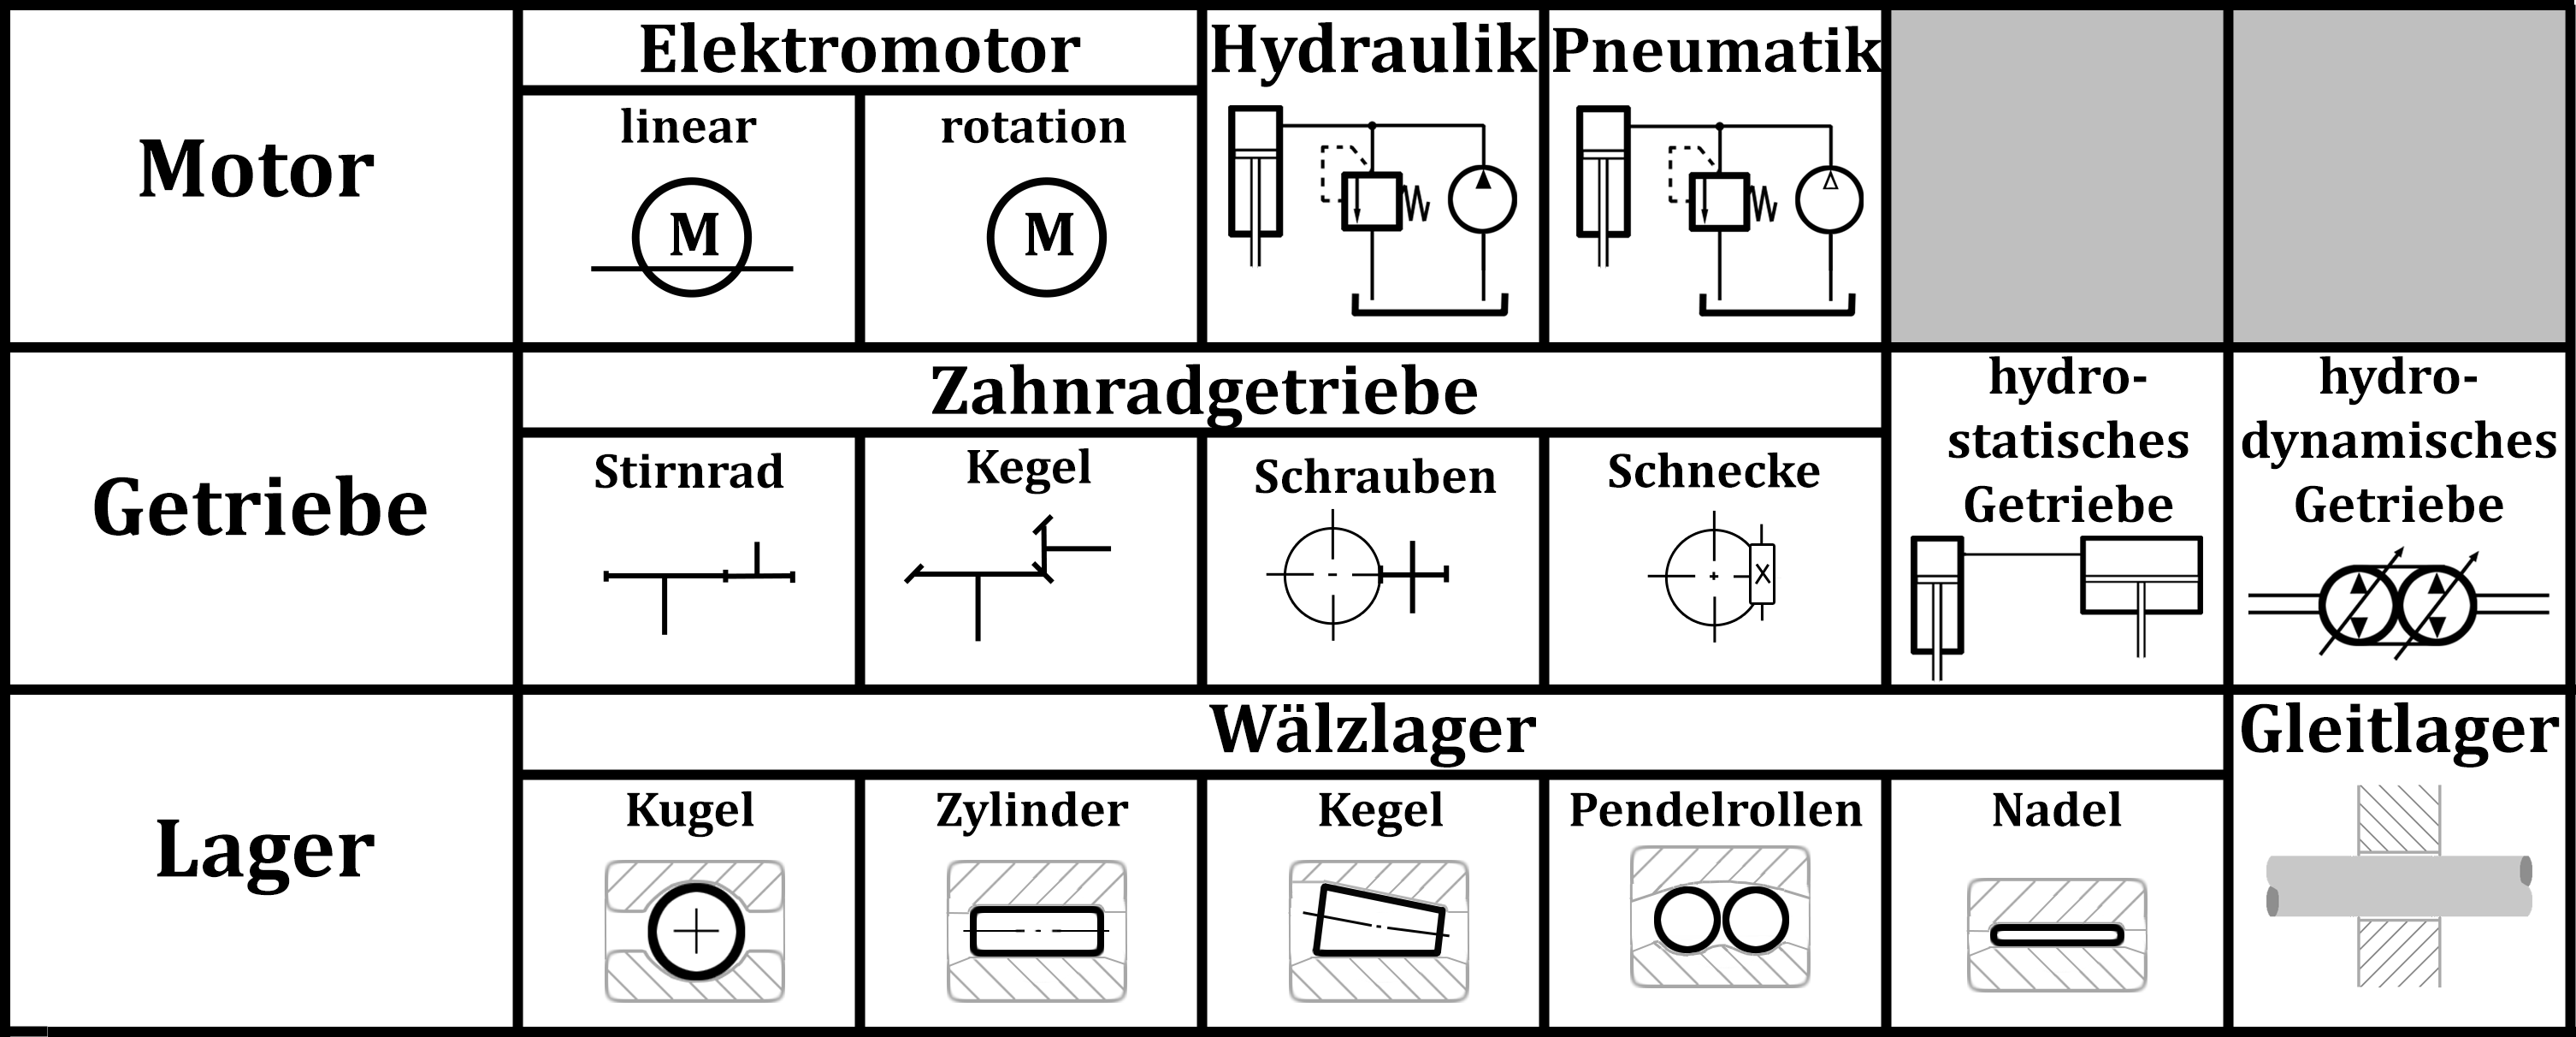
\includegraphics[width=\textwidth]{Morphologischer Kasten Ak.png}
	\caption{Morphologischer Kasten für die Grid Fin Aktuatorik}
	\label{abb_MorphKastAk}
\end{figure}
\newpage
\section{Komponentenrecherche und -auswahl}
Als nächstes werden nun die Ergebnisse der Komponentenrecherche beschrieben und auf Grund der Systemanforderungen mit Hilfe der morphologischen Kästen eine vorläufige Wahl getroffen.
\subsection{Materialwahl}
Es stehen vier verschiedene Werkstoffe zur Auswahl, die sowohl für die Raumfahrt, als auch additive Fertigung in Frage kommen: Edelstahl, Inconel (eine Nickellegierung), Aluminium- und Titanlegierungen. Tabelle \ref{tab_Werkstoffe} im Anhang zeigt Vertreter dieser Werkstoffgruppen, wie sie vom 3D-Druck-Anbieter EOS benutzt werden, und vergleicht ihre Eigenschaften. Die vielversprechendsten Vertreter der jeweiligen Werkstoffgruppen, oder jede zu denen genügend Daten vorliegen, sind zusätzlich der Übersicht halber ein weiteres Mal in Tabelle \ref{tab_WerkstoffeKlein} dargestellt.
\\~\\
Eine wichtige Eigenschaft ist natürlich die Dichte $\rho$. Hier liegen die Aluminiumlegierungen ganz klar vorne mit nur $2,57$g/cm$^3$, aber auch Titan bietet vergleichsweise gute Werte. Die Edelstähle und Nickellegierungen hingegen sind deutlich schwerer, was wiederum zu einer geringeren Wirtschaftlichkeit der Rakete führen würde, da die Masse stattdessen als Nutzlast genutzt werden könnte. Die Dichte alleine ist jedoch nicht sehr aussagekräftig, da bei geringerer Festigkeit auch dickere Strukturen benötigt werden. So zeigt Tabelle \ref{tab_Werkstoffe} zusätzlich die Streckgrenze $R_{p,0.2}$. Pro Werkstoff sind hier zwei Werte angegeben, da durch die additive Fertigung die Homogenität verloren geht, sodass die Festigkeit in den Schichten höher ist als senkrecht zu ihnen. Nur der hier ausgewählte Edelstahl hat vernachlässigbare Inhomogenitäten. Die Werte sind in Tabelle \ref{tab_WerkstoffeKlein} für alle Werkstück direkt nach der Fertigung außer beim Inconel. Mit einer thermischen Nachbearbeitung können die Streckgrenzen noch etwas erhöht und die Inhomogenitäten abgeschwächt werden. Es zeigt sich, dass die Festigkeiten der Materialien weit auseinander gehen. So kann zum Beispiel Aluminium fast nur 20\% der maximal Belastung von Titan aushalten. Um nun die beiden Aspekte der Dichte und Streckgrenze miteinander zu verbinden wird die spezifische Festigkeit $R_\mathrm{spez.}=\frac{R_{p,0.2}}{\rho}$ , also die Streckgrenze im Bezug auf die Masse, eingeführt. Es wurde der untere Wert der Streckgrenze verwendet und wenn verfügbar ohne Wärmebehandlung. Hier hebt sich Titan mit $R_\mathrm{spez.}=254$Nm/g klar von den anderen ab, während Aluminium trotz der geringen Dichte von den anderen Werkstoffgruppen großteils übertroffen wird. Hier sei auch anzumerken, dass der Vorsprung von Inconel über den Edelstählen auf die Verwendung der Materialwerte bei Wärmebehandlung zurück zu führen sind. Rechne man die spezifische Festigkeit des in diesem Kapitel dargestellten Stahls 1.4542, so erhält man einen noch besseren Wert von $R_\mathrm{spez.} = 162,0$Nm/g. Die Materialwerte von Titan scheinen sich zwar nicht groß durch eine Wärmebehandlung zu ändern, jedoch ist der Werkstoff in dieser Bewertungskategorie dank der geringen Dichte noch immer deutlich überlegen.
\\~\\
Auch wenn die Maximierung der spezifischen Festigkeit und somit eine Minimierung der Masse eine Senkung der Kosten zur Folge hat, ist der Materialpreis nicht zu vernachlässigen. Es lässt sich zwar kein genauer kg-Preis festlegen, da die entstehenden Kosten am Ende von der genauen Geometrie des Bauteils abhängen, dennoch kann eine qualitative Einordnung der verschiedenen Materialien vorgenommen werden. Hierzu wurden von der Rapidobject GmbH für die Fertigung eines Grid Fins Modells ($V \approx 100\mathrm{mm}^3$) mit verschiedenen Materialien erstellt. Dieses Modell ist etwas kleiner, als das spätere Endprodukt und auch die Geometrie steht noch nicht fest. Es zeigt dennoch gut die preislichen Unterschiede der Werkstoffe.
SO hat zum Beispiel Aluminium mit nur $1.508,9$€ die mit Abstand geringsten Kosten, während Titan das doppelte kostet. Der Edelstahl und Inconel liegen beide eng aneinander dazwischen.
\\~\\
Nicht zur die mechanische Belastbarkeit der Materialien ist entscheidend, sondern natürlich auch die thermische, um die extremen Temperaturen des Wiedereintritts zu überstehen. Hierfür muss ein Blick auf die maximale Einsatztemperatur $T_\mathrm{E, max}$ geworfen werden. Dies ist die Temperatur, bei der die mechanischen Eigenschaften des Werkstoffs stark abnehmen, sodass nicht mehr sein volles Potenzial genutzt werden kann. Aus Mangel an Daten wurde jedoch für Titan hier die Temperatur, bei der Warmumformung stattfindet, verwendet. Bei dieser Temperatur sind die Metalle weich genug, um sie verarbeiten zu können. Die wahre maximale Einsatztemperatur sollte also etwas niedriger liegen. Diese darf jedoch nur nicht langfristig überschritten werden, sodass bei der kurzen Wiedereintrittsphase auch höher Temperaturen auftreten können, ohne zum Versagen zu führen. Ein Blick auf andere Raketen, wie zum Beispiel die Flacon 9, zeigt, dass Grid Fins aus Titan und Edelstahl in diesem Fall den Bedingungen standhalten während es bei Aluminium Grid Fins zum Verlust der Form kam. Um also eine bessere Vergleichbarkeit zu erreichen, wurde zusätzlich auch noch die Schmelztemperatur aufgelistet.
\begin{table}[h] 
	\centering 
	\begin{tabular}{c|c|c|c|c|c|c|c} 
		Werkstoff&Bezeichnung&$\rho$/$\frac{k\mathrm{g}}{\mathrm{cm}^3}$&$R_{p,0.2}$/MPa&$R_\mathrm{spez.}$/Nm/g&Preis/€&$T_\mathrm{E, max}$/$^\circ$C&$T_\mathrm{Schmelz}$/$^\circ$C\\ 
		\hline 
		Aluminium&AlSi10Mg&2,57&230-270&89,5&1.508,93&530&557\\ 
		Edelstahl&1.4542&7,79&861-861&110,5&2.559,27&550&1400\\ 
		Inconel&IN 718&8,15&1140-1245&140,5&2.597,71&700&1260\\ 
		Titan&TiAl6V4&4,41&1120-1140&254,0&3.085,12&>700&1630\\ 
	\end{tabular} 
	\begin{flushright} 
		\flushbottom{Quellen: \cite{eos, preise, T1.1, T1.4, T2.1, T2.4, T2.3, T3.5, T3.8}} 
	\end{flushright} 
	\caption{Vergleichsdaten der unterschiedlichen Werkstoffe (Auswahl)}
	\label{tab_WerkstoffeKlein}
\end{table} \\
Aluminiumlegierungen zeigen bei der thermischen Belastbarkeit sehr große Schwäche, was sie für diese Anwendung zu ungünstigen Kandidaten macht. Die Titanlegierungen hingegen haben zwar mit einer extrem hohen spezifischen Festigkeit $R_\mathrm{spez.}$ ein exzellentes Leichtbaupotenzial und auch ihre ertragbaren Temperatur sind unschlagbar, sodass sie eigentlich ideale Kandidaten als Werkstoff für Grid Fins sind. Titan hat jedoch einen enormen Nachteil, was den Preis betrifft. Für einen kleinen Microlaucher, der sich gegenüber vielen Konkurrenten durchsetzten muss, ist Preis ein sehr großer Faktor der Titan als Material disqualifiziert. Edelstahl und Inconel hingegen überzeugen mit ähnlichen Werten, so ist der Preis für diese beiden Werkstoffe beinahe identisch. Wir für beide Materialien der wärmebehandelte Zustand betrachtet, hat der Edelstahl 1.4542 zwar einen höheren Wert, die maximale Einsatztemperatur $T_\mathrm{E, max}$ ist nach Angaben der Rapidobject GmbH für Inconel 718 höher \cite{preise}. Da jedoch die Schmelztemperaturen auf ähnlich hohem Niveau liegen und Anwendungsbeispiele wie die Grid Fins der Falcon 9 zeigen, dass die Einsatztemperatur von Edelstahl hoch genug liegt, sind die $\Delta R_\mathrm{spez.} = 21,5$Nm/g ein wichtigere Vorteil. Die Grid Fins werden folglich aus \textbf{Edelstahl 1.4542} hergestellt.
\subsection{Gitterdesign}
Für den Design des Gitters wird eine Auswahl der einzelnen Komponenten aus dem morphologische Kasten in Abbildung \ref{abb_MorphKastGF} getroffen.
\\~\\
Als erster Punkt werden dort verschiedene Zellformen dargestellt. Wie im Grundlagenkapitel in Abschnitt \ref{sec_zellform} dargelegt, hat die Zellform so gut wie keinen Einfluss auf die Aerodynamik. Nur im Transschall erzeugt die Wabenstruktur weniger Normalkraft. Dies kann jedoch vernachlässigt werden, da nur Machzahlen $Ma_\infty >2$ relevant ist, weil unterhalb der Ballute auslöst und die Grid Fins nicht mehr relevant sind. Bei traditionellen Fertigungsverfahren ist es in den meisten Fällen einfacher und somit günstiger die Struktur aus geraden Elementen zu fertigen. Bei der additiven Herstellung ist dieser Aspekt jedoch irrelevant, sodass nur die strukturmechanischen Eigenschaften der Zellform relevant sind. Da in den meisten Fällen \textbf{viereckige Zellen} mit maximal \textbf{dreieckigen Seitenelementen} benutzt wurden, wird auch diese praxiserprobte Variante gewählt. Zudem gibt es hierzu die meisten Daten, was die Wahrscheinlichkeit von unerwartetem Verhalten minimiert.
\\~\\
Auch für die Gitterform gibt es unterschiedliche Möglichkeiten. Da jedoch keine Studien über ihren Einfluss auf die erzeugbaren Kräfte existieren, muss auch hier in anderer Hinsicht argumentiert werden. Um den rechteckigen Baumraum eines 3D-Drucker ideal nutzen zu, bietet sich auch eine rechteckige Gitterform an. Dies ermöglicht eventuelle einen kleineren Drucker zu nutzen und somit Fertigungskosten einzusparen. Auch auf diese Form lässt sich die Zuspitzung des Grid Fins, wie sie bei den anderen beiden Varianten zu sehen ist anwenden, um einen besseren Kraftfluss zu ermöglichen. Zusätzlich lassen sich durch additive Fertigung die Außenkanten ohne großen Mehraufwand wie beim Insektenflügel abrunden, was die Struktur weiter entlasten sollte. Somit ist die Wahl auf ein \textbf{Rechteckgitter} mit \textbf{Zuspitzung zur Einspannung} hin und \textbf{abgerundeten Außenkanten }gefallen.
\\~\\
Die Wandquerschnittsform hat im Gegensatz zu den anderen beiden bisherigen Aspekten einen großen Einfluss auf die Aerodynamik oder genauer gesagt den Widerstand. Dieser Effekt wurde im Grundlagenkapitel in Abschnitt \ref{sec_wandquerschnitt} behandelt. Auch wenn Widerstand nicht zwangsläufig negativ zu bewerten ist, da die Rakete so beim Wiedereintritt stärker abgebremst wird, bedeutet mehr Widerstand auch mehr Belastung, also kürzere Lebensdauer beziehungsweise schwererer Grid Fin. Der Mehraufwand von komplexeren Querschnittsformen fällt durch die additive Fertigung auch weg. So wird für das \textbf{Gitter} eine \textbf{beidseitig spitze} Form gewählt, wegen des geringeren Widerstandes. Für den \textbf{Rahmen} wird die \textbf{Trapezform} verwendet, da die Außenkante flach sein kann. Es wurde sich gegen die Dreiecksform entschieden, obwohl die den geringsten Widerstand liefert, da weniger Material außen ist und somit schlechter Biegemomente um eine horizontale Achse aufgenommen werden können. Des Weiteren ist der Effekt auf die Normalkraft, wenn nur angeschrägte Flachen existieren unbekannt.
\\~\\
Auch die Krümmung hat wieder eine vernachlässigbar kleinen Einfluss auf die Aerodynamik von Grid Fins. Durch die additive Fertigung im 3D-Drucker ist auch kein wirklicher zusätzlicher Aufwand damit verbunden. Um beim Wiedereintritt den Grid Fin nicht gegen die Widerstandskraft halten zu müssen, soll er zum Triebwerk hin angelegt werden. Somit wird der Grid Fin mit einer zur Anströmung \textbf{konkaven Krümmung} modelliert.
\\~\\
Mit einer Pfeilung lässt sich nun wiederum die wirkenden Axialkräfte verändern. Mit der konfigurellen Pfeilung lassen sich diese Kräfte um bis zu das 4-fache erhöhe. Dies würde zu einer deutlich stärkeren Belastung führen, wodurch der Grid Fin stabiler und somit schwerer und unwirtschaftlicher wird. Sollte nun hingegen eine verstellbare konfigurelle Pfeilung implementiert werden, so steigen die Anforderungen an den Aktuator wieder deutlich an. Dies würde zu einer deutlichen Kostensteigerung führen ohne signifikante Vorteile, da der restliche Körper noch immer deutlich größere Anteile zum aerodynamischen Widerstand liefert. Somit wir eine Pfeilung der Konfiguration an dieser Stelle ausgeschlossen.

Die Pfeilung des Gitters ist wiederum nicht mit der Krümmung verträglich. Das bessere Anlegen des Grid Fins an die Außenhülle der Rakete ist an dieser Stelle der Widerstandsreduzierung einer solchen Pfeilung vorzuziehen.

Bleibt nun also nur noch die lokale Pfeilung, welche keinen Einfluss auf andere Designparameter hat. Auf der Außenseite, beziehungsweise der Stromabwärtsseite, kommt sie jedoch auch nicht in Frage, da sie im eingeklappten Zustand beim Raketenstart in die Strömung ragt und somit zusätzlichen Widerstand verursachen würde. Auf der \textbf{luv-Seite} hingegen ist die \textbf{lokale Pfeilung} eine gute Möglichkeit der Widerstandsreduzierung und wird deswegen implementiert. Die wohl bekannteste Verwendung der lokalen Pfeilung befindet sich an den Grid Fins der Falcon 9, welche den Berg-Typus verwendet. Die Analysen von Guyot und Schülein \cite{PeakValley}, dass, auch wenn beide Varianten den gleichen Widerstandsvorteil habe, die Normalkraft, bei dem Tal-Typus jedoch höher ist. Da die Grid Fins von SpaceX aber auch keine spitze Vorderkante haben, würden bei ihnen eine lokale Pfeilung des Tal-Typus an den Schnittstellen nahezu zu einer Sackgasse für die Strömung kommen, was einen großen Widerstand bewirkt. Da bei diesem Grid Fin die Gitterwände eine doppel-spitzen Wandquerschnitt haben, wie es auch bei den Untersuchungen von Guyot und Schülein der Fall war, wird hier der \textbf{Tal-Typus} verwendet. Da das größte Bedenken hier die Stabilität der Zacken betrifft, die sich im Gegenteil zum Berg-Typus nicht gegenseitig stützen, kann es sein, dass nach der FEM-Anaylse der Typus noch gewechselt wird.
\subsection{Peripherie und Aktuator}
Für alle der drei Energiemedien ist sind schon Vertreter in der Rakete installiert, die unter Umständen genutzt werden könnten. Da sich die Grid Fin Aktuatorik im selben Abschnitt wie die Boardelektronik der ersten Stufe befindet, sind auch hier direkt die Batterien, mit denen Elektromotoren betrieben werden können. So wird mit ihnen zum Beispiel auch die elektrischen Treibstoffpumpen für die Triebwerke mit Strom versorgt. Somit liegt direkt auch schon ein Hochdruckfluid vor, welches als Druckmittel für die Hydraulik genutzt werden könnte. Da sich dieses jedoch am anderen Ende der Rakete befindet und dafür sowohl ein Eingriff in die komplexen Triebwerke, so wie eine Abhängigkeit von vorhandenem Treibstoff oder LOX zu Stande kommt, ist dies eine weniger plausible Möglichkeit. Sodass eine eigene elektrische Pumpe und Druckmittel eine realistischere Umsetzung für eine Hydraulik wären. Für eine Pneumatik könnte jedoch ein vorhandenes System genutzt werden. Der Heliumtank für den Druckausgleich in den Tanks liegt direkt unterhalb der Elektronik und es existieren sogar schon Leitungen, die das Gas in diesen Bereich der Rakete für das RCS transportieren.
\\~\\
Da sowohl für den Klappwinkel, als auch den Steuerwinkel unterschiedliche Anforderungen existieren, die auch andere Lösungsmöglichkeiten zulassen, werden diese im Folgenden getrennt betrachtet.
\subsubsection{Klappwinkel}
\subsubsection{Steuerwinkel}
\subsection{Getriebe und Lagerung}

\section{Festlegung des Modelldesigns}\label{sec:modelldesign}
Nun da das Design feststeht, muss nur noch die Größe der einzelnen Parameter festgelegt werden. Die Größe der Querschnittsfläche $A$ ist abhängig von der Auftriebserzeugung, die gewährleistet werden soll. Aus der Simulation ist bekannt, dass ungefähr
\begin{equation}
	A \cdot C_{N\alpha}= 0,00432 \mathrm{m}^2/^\circ
\end{equation}
bei einer Machzahl von $Ma_\infty = 2.0$ und $\alpha = 0^\circ$ gelten soll. Da die einzelnen Modellierungsparameter hauptsächlich einen Einfluss auf den Widerstand haben und die Normalkraft, wir von einem ähnlichen Wert von $C_{N\alpha}$ ausgegangen, sodass auch eine Fläche von $A=0,9\mathrm{m}^2$ benötigt wird.

Das Verhältnis von Zellgröße zur Sehnenlänge kann jedoch den Auftriebsbeiwert verändern. Da aber nur Studien zum niedrigen Unterschall, bei denen ein Maximum bei gleicher Länge dieser beiden Parameter erreicht wird, wird hier ein Blick auf die bisher verwendeten Grid Fins geworfen. Wie Abbildung \ref{abb_f9_GF} zu erkenn gibt verwendet SpaceX bei seiner Falcon 9 auch ein Verhältnis von ungefähr 1:1, während Chinas Chang'e eine etwas kleinere Zellgröße zu besitzen scheint (vgl. Abbildung \ref{abb_change}). Da jedoch die Grid Fins in den meisten Studien die gleiche Zellgröße wie Sehnenlänge haben, lässt dies vermuten, dass die auch im Überschall dadurch die höchsten Normalkraftwerte erzeugt werden. Also wird auch hier dieses Verhältnis verwendet und der Wert $C_{N\alpha}$ und somit auch die Fläche müssen nicht verändert werden. Nun wird aus gängigen Werten für die Sehen ein Wert für diese festgelegt, sodass die zwei Parameter mit $\mathbf{s=g=0,04m}$ festgelegt werden.

Bei der Höhe $h$ und Breite $b$ können nun Werte gewählt werden, die ganzzahlig durch die Diagonale in der Zelle teilbar ist. Wird nun ein Seitenverhältnis von 5:6 gewählt, was zu einer Höhe von $\mathbf{h= }6\cdot g\sqrt{2}=\mathbf{339,4mm}$ und einer von $\mathbf{b= }5\cdot g\sqrt{2}=\mathbf{282,8mm}$ führt. Dies muss auch in den Bauraum eines Druckers passen. Dieser hat zwar nur eine Grundfläche von 300x300mm$^2$, aber da er 400mm hoch ist kann dich Diagonale von 500mm genutzt werden, indem in diese Eben auch die Höhe des Grid Fins gelegt wird. Die Fläche die durch die Höche und Breite des Grid Fins aufgespannt wird liegt mit $0,096\mathrm{m}^2$ noch etwas über der angestrebten Fläche. Jedoch muss diese noch um die vier halbe Zellen reduziert werden, da sich die Geometrie zur Einspannung hin schmälern soll. Übrig bleibt eine Fläche von $A=h\cdot b-2g^2=0,0928\mathrm{m}^2$.

Da sich an der Wanddicke $d$ im Laufe der FEM-Simulationen vermutlich am meisten ändern wird, soll an dieser Stelle nur ein kurze Überschlagsrechnung gemacht werden. Angenommen wird, dass die Wandstärke nicht in der Gitterform über die Breite verteilt ist, sondern alle zusammen addiert einen Balken mit der Gesamtdicke $d_\mathrm{ges.}(x_h)$ bilden. $x_h$ ist hierbei eine Koordinate die sich über den Grid Fin in Höhenrichtung spannt mit $x \epsilon [0, h]$. Dieser wird nur durch die maximale Kraft in Sehnenrichtung gleichmäßig auf der gesamten Länge $h$ und Breite $d_\mathrm{ges}(x_h)$ belastet. Die Kraft in Sehnenrichtung $F_s$ wird aus dem maximalen Kraftvektor in Gleichung \ref{eq_Fmax} bestimmt. Dieser ist im körperfesten Koordinatensystem gegeben, sodass er bei einem Steuerwinkel von $\delta = 10^\circ$ und in x-Konfiguration $\lambda=45^\circ$ noch wie folgt umgerechnet werden muss.
\begin{equation}
	F_s = F_x\cos{\delta}+\sqrt{F_y^2+F_z^2}\sin{\delta}
\end{equation}
Es bildet sich ein Momentenverlauf 
\begin{equation}
	M(x_h) =\frac{F_{s}}{d_\mathrm{ges.}}\left(-\frac{1}{2}x_h^2+hx_h-\frac{1}{2}h^2\right)
\end{equation}
aus. Die größte Spannung herrscht in der äußersten Faser bei
\begin{equation}
	 \sigma(\pm \frac{s}{2}, x_h)=\frac{6M(x_h)}{s^2d_\mathrm{ges.}}.
\end{equation}
Wie dick nun für die jeweiligen x-Werte die Zellwände insgesamt sein müssen, hängt von der Festigkeit des Materials ab.
\begin{equation}
	R_{p, 0.2} \geq\sigma_\mathrm{max}
\end{equation}
Somit ergibt sich die Gesamtdicke zu
\begin{equation}
	d_\mathrm{ges}\geq \sqrt{\frac{6F_{s}\left(  -\frac{1}{2}x_h^2+hx_h-\frac{1}{2}h^2\right)}{R_{p, 0.2}s^2}}
\end{equation}
Wir nun noch ein Sicherheitsfaktor von 1,5 dazu multipliziert, da die Kraftanteile in Breiten- und Höhenrichtung nicht mit einbezogen wurden, erhält man den Verlauf der einzelnen Wandstärken $d(x_h)$, indem die Gesamtdicke gleichmäßig auf die zwei Rahmenwände und fünf Schnittstellen der Gitterwände verteilt wird.
\begin{figure}[h]
	\centering
	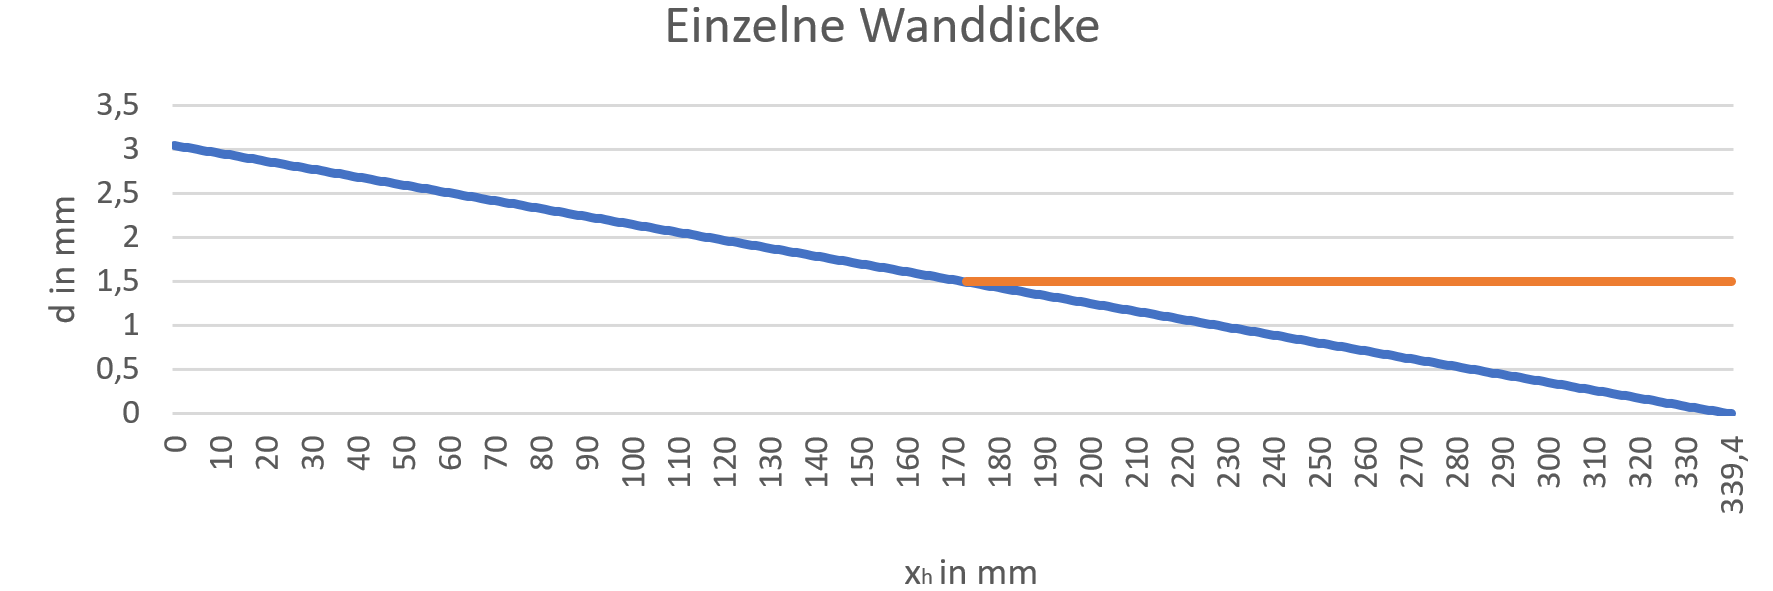
\includegraphics[width=0.85\textwidth]{d_einzel.png}
	\caption{Der Verlauf der Wanddicke $d$ in Abhängigkeit von $x_h$}
	\label{abb_d_einzel}
\end{figure}\\
Da das Moment unter diesen einfachen Annahmen am Ende des Grid Fins auf null fällt, errechnet sich dort auch ein Wandstärke von null. Dies ist natürlich kein sinnvolles Ergebnis, sodass eine minimale Wanddicke von $d_\mathrm{min}=1,5$ mm definiert wird. Des Weiteren ist noch zu beachten, dass die Dicke in der Nähe der Einspannung noch höher als dargestellt ist, da dort weniger Wände liegen, auf die die Gesamtdicke verteilt wird.
\\~\\
Nun steht schon mal eine erste Geometrie des Grid Fins, jedoch benötigen auch die zusätzlichen Designelement, die aus dem morphologischen Kasten gewählt wurde Festlegung weitere Werte. Einer davon ist der Pfeilungswinkel $\Lambda_\mathrm{lokal}$. Je größer dieser ist, desto geringer ist die axiale Kraft, doch große Pfeilung schwächt gleichzeitig die Sehne in den Tälern. Also Kompromiss wird der Pfeilungswinkel variiert. An den \textbf{Spitzen} soll ein $\mathbf{\Lambda_\mathrm{lokal}=70^\circ}$ gelten in den Tälern jedoch nur $\Lambda_\mathrm{\textbf{lokal}}=20^\circ$. Der Berg soll $20$mm höher liegen als das Tal und verbunden werden sie über einen Tangentenbogen. Die Fläche dieser Pfeilung entspricht einem Rechteck gleicher Breite mit der Höhe $7$mm. Um also auf eine Sehnenlänge von $s=40$mm zu kommen, muss sich noch $33$mm restliche Wand unter der Pfeilung befinden.

Der Wandquerschnitt spitzt sich auch zu und der zugehörige Winkel wurde für das Gitter auf $70^\circ$ gesetzt. Die Position in wieder so gewählt, dass die durchschnittliche Sehnenlänge sich immer auf dem Wert befindet, der durch die lokale Pfeilung herrschen sollte. Die Rahmenwände haben nur auf einer Seite eine schräge. Der Winkel wurde hier auf\ $54^\circ$ herab gesetzt, sodass Rahmen und Gitter bei gleicher Wandstärke und Sehnenlänge, die selbe maximale Höhe haben.
\begin{figure}[h]
	\begin{minipage}[t]{0.45\linewidth}
		\centering
		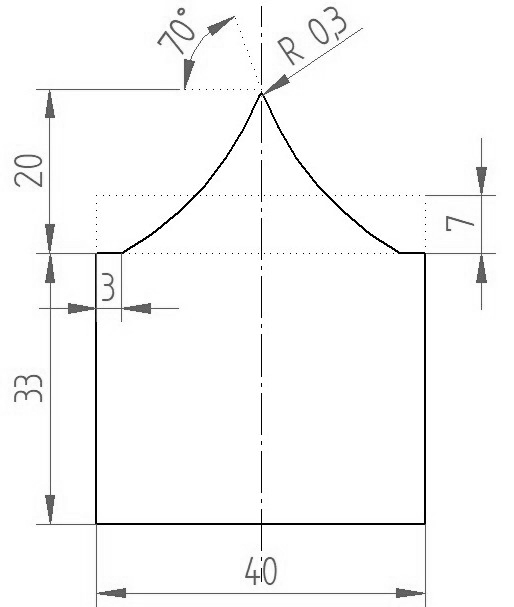
\includegraphics[width=0.85\textwidth]{Pfeil_lok.png}
		\caption{Die Geometrischer Zusammenhänge einer gepfeilten Zellwand}
	\end{minipage}
	\hfill
	\begin{minipage}[t]{0.45\linewidth}
		\centering
		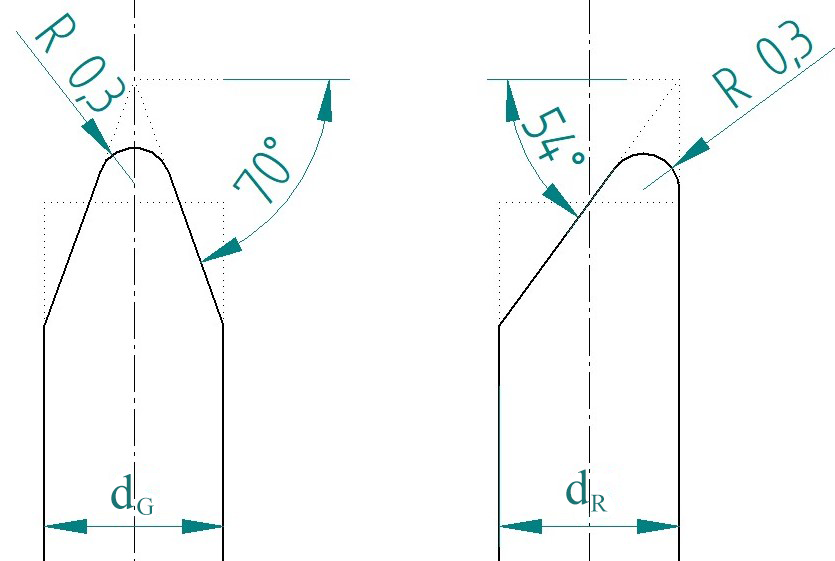
\includegraphics[width=\textwidth]{Wandquerschnitt.png}
		\caption{Zuspitzung der Wände im Querschnitt}
	\end{minipage}
\end{figure}\\
Die Krümmung soll für die Vorderkante der nominellen Sehne ausgelegt werden, also für den Fall, dass keine Pfeilung oder Zuspitzung vorliegt (gepunktete Linie). Da an den Bergen der Pfeilung die Spitze $13$mm und mit der Zuspitzung bei eine Wandstärke von $4$mm einen weiteren Millimeter über der nominelle Sehne liegt, müssen noch mindestens $14$mm auf die $550$mm Raketenradius drauf addiert werden. Somit wird der Krümmungsradius auf $570$mm gesetzt.
\\~\\
Es sind noch weitere Optionen möglich, mit denen sich die Grid Fins modifizieren lassen würden. Diese werden hier jedoch zunächst nur kurz vorgestellt und erst nach den ersten Analysen beurteilt, ob sie eventuell doch noch implementiert werden sollen.

Die additive Fertigung des Grid Fins ermöglicht neue Optionen, die für klassische Herstellungsverfahren nicht wirtschaftlich umsetzbar sind. So können zum Beispiel Kanäle in das Material integriert werden, welche genutzt werden können, um den Werkstoff zu kühlen oder gar das Air Flush System mit weiteren Drucksensoren ergänzen. Es wäre auch denkbar diese einfach nur zur weiteren Gewichtsreduzierung zu nutzen.

Auch denkbar ist es die scharfen Kanten, die senkrecht zur Strömung liegen, abzurunden und so einen besseren Kraftfluss zu erlauben.
\\~\\
Zum Schluss muss an dieser Stelle noch angemerkt werden, dass 3D-Drucker natürlich nur eine begrenzte Auflösung haben. Je nach Hersteller kann somit die minimale Wandstärke $0,4-1,0$mm \cite{eos, preise} und die Schichtdicke $0,04-0,075$mm \cite{preise} betragen. Die Ausrichtung im Drucker hat also auch Einfluss auf den Detailgrad. Somit kann es sein, dass die spitzen Kanten und die Pfeilung in der Fertigung stumpfer werden, als sie ausgelegt wurden. Auch das Hinzufügen von Kanälen ist nur möglich, wenn die Wände dick genug sind.
\section{Modellierung des Modells}
Nun wo das Design feststeht, soll es auch in einem CAD-Programm modelliert werden. Hier wird Solid Edge der Siemens PLM Software Inc.. Zunächst wird eine Skizze angefertigt, die den Grundriss des Grid Fins zeigt. Aus dieser wird dann ein Volumen extrudiert. Dabei wir ein viel zu großes Maß gewählt, da Sehenlänge erst im nächsten Schritt festgelegt wird.
\begin{figure}[h]
	\centering
	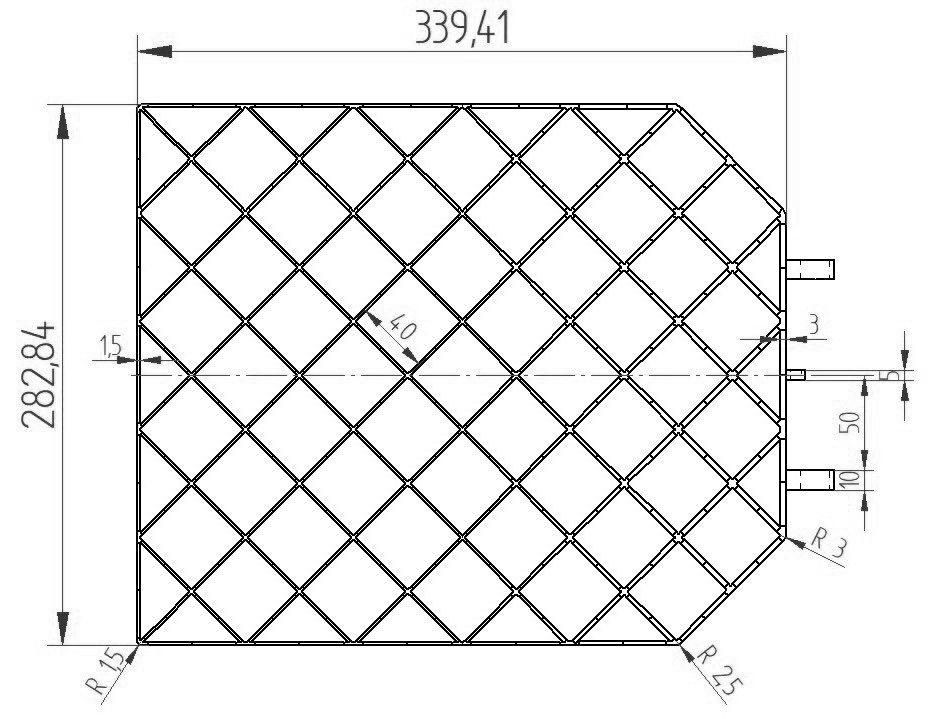
\includegraphics[width=0.85\textwidth]{grundriss.jpg}
	\caption{Grundrissskizze des Grid Fins in Solid Edge}
	\label{abb_grundriss}
\end{figure}\\
Als nächstes wird die senkrecht zu der Ebene, in der der Grundriss liegt eine neue Skizze angefertigt. Diese zeigt den Durchmesser des Raktenkörpers so weit ausgedehnt, dass er dem Krümmungsradius von $570$mm entspricht. Ein zweiter Kreis mit dem selben Radius wird um $34$mm nähere an den Grid Fin gelegt. Nun wird anhand dieser Skizze der Grundriss ausgeschnitten, sodass nur noch der Teil zwischen den beiden Kreisen übrig bleibt. Das Ergebniss ist ein sowohl außen, als auch innen, geilchmäßig gekrümmter Grid Fin mit einer konstanten Sehenelänge von zunächst $34$mm.
\begin{figure}[h]
	\centering
	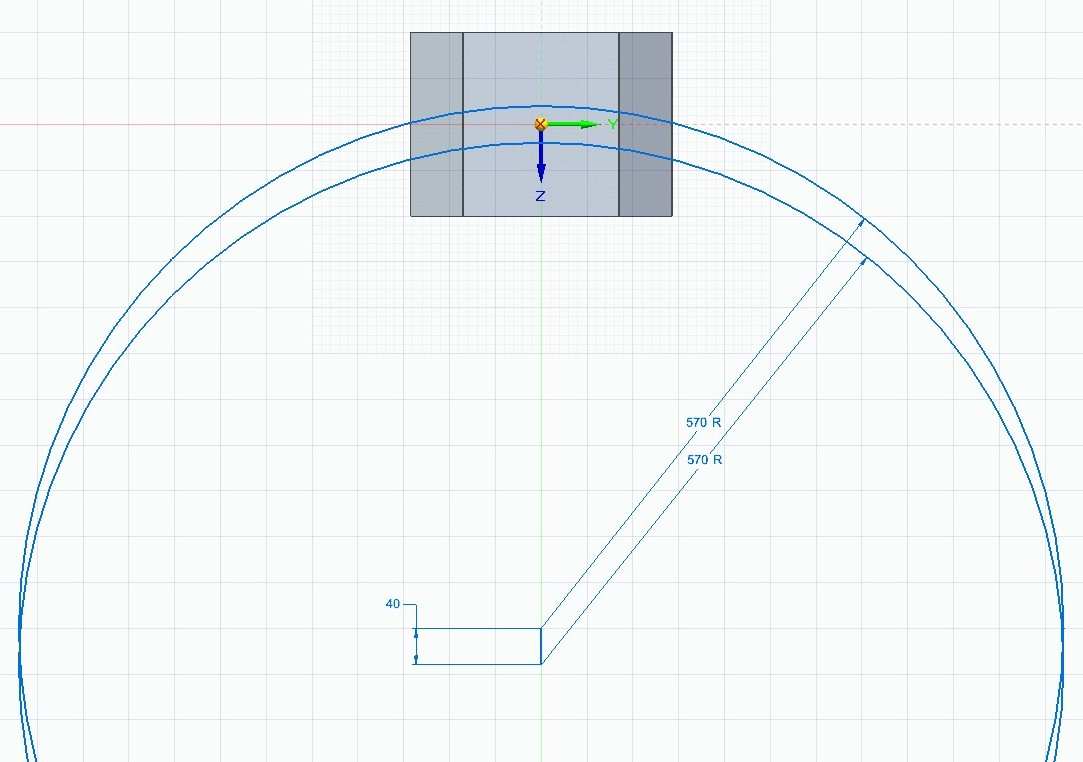
\includegraphics[width=0.85\textwidth]{körper.jpg}
	\caption{Krümmungsskizze des Grid Fins in Solid Edge}
	\label{abb_körper}
\end{figure}\\
Im nächsten Schritt wird die konvexe Seite des Grid Fins bearbeitet. Hier fehlt nur noch die Zuspitzung der Wandquerschnitte. Hierzu werden an den Kanten, beim Gitter beidseitig und am Rahmen nur innen, Fasen mit dem entsprechenden Winkel angebracht. Dadurch wird im Schnitt die Sehenlänge auf $33$mm reduziert.